\scanpage{119}
\mspage{110}
% archive sheet number: 119 (lower left)
% Heading
\uline{Parenthèse} Zoologie des \uline{sommets} d'une préfigure.

% upper-left drawing
\figure{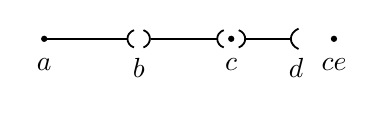
\begin{tikzpicture}[line width=.65pt]
\draw (0,0)--(1.05,0); \draw (1.35,0)--(2.2,0); \draw (2.55,0)--(3.15,0);
\fill (0,0) circle (.04); \fill (2.375,0) circle (.04); \fill (3.68,0) circle (.04);
\draw (1.14,.11) .. controls (1.03,.07) and (1.03,-.07) .. (1.14,-.11);
\draw (1.26,.11) .. controls (1.37,.07) and (1.37,-.07) .. (1.26,-.11);
\draw (2.28,.11) .. controls (2.17,.07) and (2.17,-.07) .. (2.28,-.11);
\draw (2.47,.11) .. controls (2.58,.07) and (2.58,-.07) .. (2.47,-.11);
\draw (3.23,.13) .. controls (3.10,.07) and (3.10,-.07) .. (3.23,-.13);
\node[below] at (0,-.12) {$a$}; \node[below] at (1.2,-.12) {$b$};
\node[below] at (2.375,-.12) {$c$}; \node[below] at (3.2,-.12) {$d$};
\node[below] at (3.68,-.12) {$\deleted{\unsure{c}}e$};
\end{tikzpicture}}
\[
\begin{aligned}
\Phi&=\{\deleted{\unsure{P}}_a,S_{ab},S_{bc},\deleted{\unsure{P}}_{\unsure{d|c}}\deleted{\unsure{\{}}S_{cd},e\}\\
\overline{\Phi}&=\{\deleted{\unsure{P}}_a,S_{ab},\deleted{\unsure{P}}_b,S_{bc},\deleted{\unsure{P}}_c,\deleted{\unsure{P}}S_{c\deleted{\unsure{b}}d},d,e\}\\
\partial\Phi&=\{a,d\}
\end{aligned}
\]
% Upper-right block: cancelled with several diagonal strokes.
\deleted{$\delta\Phi$ (ens. des sommets de $\Phi$) $=\overline{\Phi}\cap\unsure{\mathcal{L}|L}=(\overline{\Phi})_0$}

\deleted{sommets \uline{propres} : $\delta\Phi\cap\Phi_0$, \uline{impropres} $\delta\Phi\cap\mathcal{L}$}
\[
\deleted{\operatorname{ord}(\underset{\substack{\uparrow\\\mathcal{L}}}{a},\Phi)=\operatorname{card}(\{X\in\unsure{M|\mathcal{M}}\cap\Phi=\Phi_1\mid a\triangleleft X)}
\]
\[
\deleted{\delta\Phi=\{a\in\mathcal{L}\mid\operatorname{ord}(a,\Phi)=}
\]
\deleted{sommet isolé de $\Phi$ : d'ordre 0}

\deleted{sommet bord de $\Phi$ : d'ordre 1}
\[
\deleted{\text{deux cas }\left\{\begin{aligned}a\in\Phi&\quad\text{sommet bord propre}\\a\notin\Phi&\quad\text{sommet bord impropre}\end{aligned}\right.}
\]

% L10-14, full-width text
Rappels
\[
\delta\Phi\ (\text{ensemble des \uline{sommets} de }\Phi)=\overline{\Phi}\cap\mathcal{L}=(\overline{\Phi})_0
\]
sommets \uline{propres} : ceux de $\Phi_0=\overline{\Phi}\cap\mathcal{L}\subset\delta\Phi$

sommets impropres : ceux qui ne sont pas dans $\Phi_0$
\[
\operatorname{ord}(\underset{\substack{\uparrow\\\mathcal{L}}}{a},\Phi)=\operatorname{card}(\{X\in\underset{\inserted{\substack{\Vert\\M\cap\mathcal{L}}}}{\Phi_1}\mid a\triangleleft X)\in\{0,1,2\}.
\]
% L15-17
(\uline{ordre de} $a$ \uline{p.r. à} $\Phi$) Cet ordre est zéro si $a$ n'est pas un sommet, mais il peut être zéro aussi pour un sommet de $\Phi$, \deleted{\unsure{car}}

% L18-20
\uline{Lemme} Si $a\in\delta\Phi$, \deleted{alors}\inserted{et} $\operatorname{ord}(a,\Phi)=0$, on a $a\in\Phi$.
Un tel sommet de $\Phi$ est dit \deleted{\unsure{isolé}}\uline{sommet isolé}.
\[
\Phi_{\mathrm{is}}=\{a\in\delta\Phi\mid\operatorname{ord}(a,\Phi)=0\}\subset\Phi_0
\]
% L21-25
Les sommets d'ordre 1 sont les \uline{sommets-bord}
\[
\partial\Phi=\{\underset{\inserted{\text{ou }s\in\mathcal{L}}}{s\in\delta\Phi}\mid\operatorname{ord}(\unsure{a|s},\Phi)=1\}
\]
Parmi ces sommets\inserted{-bord} on distingue les sommets-bord propres, et impropres
\[
\underbrace{\Phi_0\cap\partial\Phi=\partial_0\Phi}_{\substack{\text{sommets-bord}\\\text{propres}}}\subset\Phi
\]
\deleted{\unsure{$P$}}

Les sommets d'ordre 2 sont les \uline{sommets} \uline{internes}
\[
\deleted{\unsure{\delta}}\delta_{\mathrm{int}}(\Phi)=\{\underset{\inserted{\text{ou }s\in\mathcal{L}}}{s\in\delta\Phi}\mid\operatorname{ord}(s,\Phi)=2\}
\]
